\chapter{Introduction}\label{ch:introduction}
This manual describes the AIDA \gls{tlu} designed for the \href{http://aida2020.web.cern.ch/}{AIDA-2020 project} by David Cussans\footnote{University of Bristol, Particle Physics group} and Paolo Baesso\footnote{University of Bristol, Particle Physics group}.\\
The unit is designed to be used in High Energy Physics beam-tests and provides a simple and flexible interface for fast timing and triggering signals at the AIDA pixel sensor beam-telescope.\\
The current version of the hardware is an evolution of the \href{https://twiki.cern.ch/twiki/bin/view/MimosaTelescope/TLU}{EUDET-TLU} and the \href{https://www.ohwr.org/projects/fmc-mtlu/wiki}{miniTLU} and is shipped in a metallic case that includes an \gls{fpga} board and the \gls{tlu} \gls{pcb}: the \gls{fpga} is responsible for all the logic functions of the unit, while the \gls{pcb} contains the clock chip, discriminator and interface blocks needed to communicate with other devices.\\
The current version of the \gls{pcb} is \brd and is designed to plug onto a carrier \gls{fpga} board like any other \gls{fmc} mezzanine board, although its form factor does not comply with the ANSI-VITA-57-1 standard.\\

\section{Overview}
The AIDA \gls{tlu} provides timing and synchronization signals to test-beam readout hardware.\\
The hardware can provide an internally generated low-jitter 40~MHz clock or can accept and external clock reference.\\
It accepts the asynchronous trigger signals from up to six external sources, such as beam-scintillators, and generate synchronous signals (including global trigger or control signals) to send to up to four devices under tests. The logic function used to generate the trigger can be defined by the user among all the possible logic combinations of the inputs.\\
Depending on the chosen mode of operation, the \gls{tlu} can accept busy signals or other veto signals from \gls{dut}s and react accordingly, for instance avoinding any further trigger until all the busy signals have been de-asserted.\\
Whenever a global trigger is generated by the unit, a 48-bit time-stamp is attached to it. This time stamp is based on the 40~MHz clock. Additionally ???\\
The configuration parameters and data are sent and received via the \href{https://www.ohwr.org/projects/ipbus}{IPbus}. IPbus is a simple way to control and communicate TCA-based hardware via the UDP/IP protocol.


\section{FPGA}
The \gls{tlu} is shipped with an \gls{fpga} board already programmed with the latest version of the firmware needed to operate the unit.\\
The firmware developed at University of Bristol is targeted to work with the Enclustra  AX3 board, which must be plugged onto a PM3 base, also produced by \href{http://www.enclustra.com/en/home/}{Enclustra}. The firmware is written on the \gls{fpga} using a \gls{jtag} interface. Typically a breakout board will be required to connect the Xilinx programming cable to the Enclustra PM3. All these components are included in the \gls{tlu} enclosure so the user can upload a new version of the firmware by simply connecting a \gls{usb}-B cable in the back panel of the unit.\\
At the time of writing this work\footnote{Oct 2017} the AX3 is the only \gls{fpga} for which a firmware has been developed. However, we plan to ship future versions of the \gls{tlu} with a custom made \gls{fpga} designed by Samer Kilani.
\begin{alertinfo}{Note}
    If the \gls{fpga} detects a programming cable connected it will not load the firmware from its memory after a power cycle.\\
    It is recommended to leave the \gls{usb} cable disconnected from the back panel unless there is the intention to re-program the firmware.
\end{alertinfo}


\section{Power}
The \gls{tlu} requires 12~V to operate. Power can be provided using the circular jack on the back panel of the unit.\\
During normal operation the current drawn by the unit is about 0.5~A.
%\section{Preparation}
%Before powering the \gls{tlu} it is necessary to follow a few steps to ensure the board and the \gls{fpga} work correctly.\\
%
%Currently, it is recommended to use the following:
%\begin{itemize}
% \item MA-PM3-W-R5: Mars PM3 base board
% \item MA-AX3-35-1I-D8-R3: Marx AX3 module (hosts a Xilinx XC7A35T-1CSG324I )
% \item MA-PM3-ACC-BASE: Accessory kit, including a \gls{jtag} breakout board to connect Xilinx programming cables. Also includes a 12~V power supply to power the PM3.
%\end{itemize}
%
%\section{I/O voltage setting}
%The I/O pins of the PM3 can be configured to operate at 2.5~V or 3.3~V; the factory default is 2.5~V but the \brd requires 3.3~V logic. The user should make sure to select the appropriate voltage by operating on DIP-switch CFG-A/S1200 (pin 1 set to ON).\\For reference, a top view of the board is provided in the appendix at page~\pageref{ch:appendix}.\\
%\begin{alertinfo}{Warning}
%    Please double check the PM3 board manual for the correct way to change the I/O voltage setting. Enclustra has been changing their hardware recently.
%\end{alertinfo}
%
%\section{Xilinx programming cable}
%The \gls{jtag} pins on the PM3 are located on the header J800 (20-way, 2.54~mm pitch). The breakout board provided by Enclustra sits on top of the header and connects the pins to a 14-way Molex milli-grid header so that it is possible to plug the Xiling programming cable directly onto it. However, when the \brd is mounted on a base plate as shown in figure~\ref{fig:TLUplate}, the breakout board has to be detached from the PM3 because it interferes with the mounting screws.\\
%The connection between J800 and the breakout can be achieved by using two standard 20-way \gls{idc} cables as shown in figure~\ref{fig:XilinxCable}.
%\begin{figure}[h]
%  \centering
%  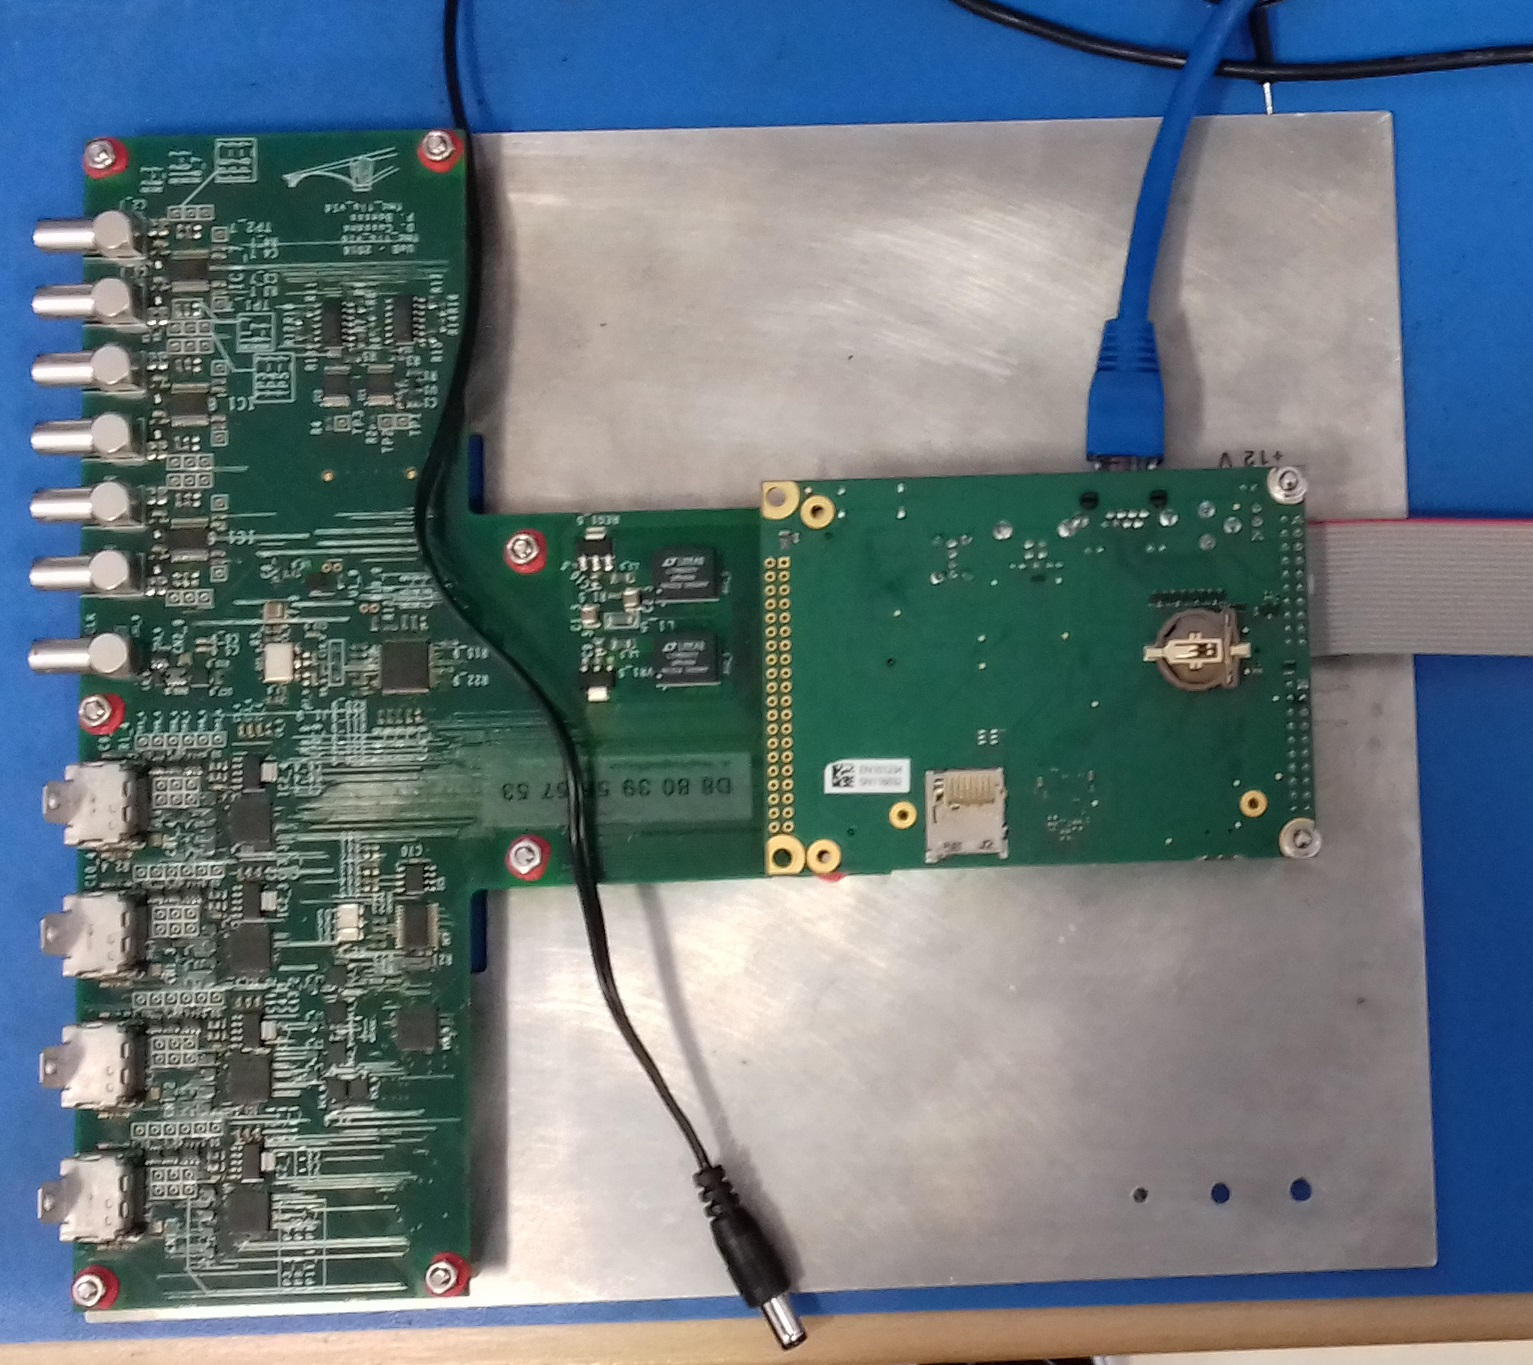
\includegraphics[width=.50\textwidth]{./Images/TLU_plate.jpg}
%  \caption{\brd and PM3 mounted on a base plate: in this configuration it is not possible to install the breakout board on the PM3 because the mountings screws are in the way.}\label{fig:TLUplate}
%\end{figure}
%\begin{figure}
%  \centering
%  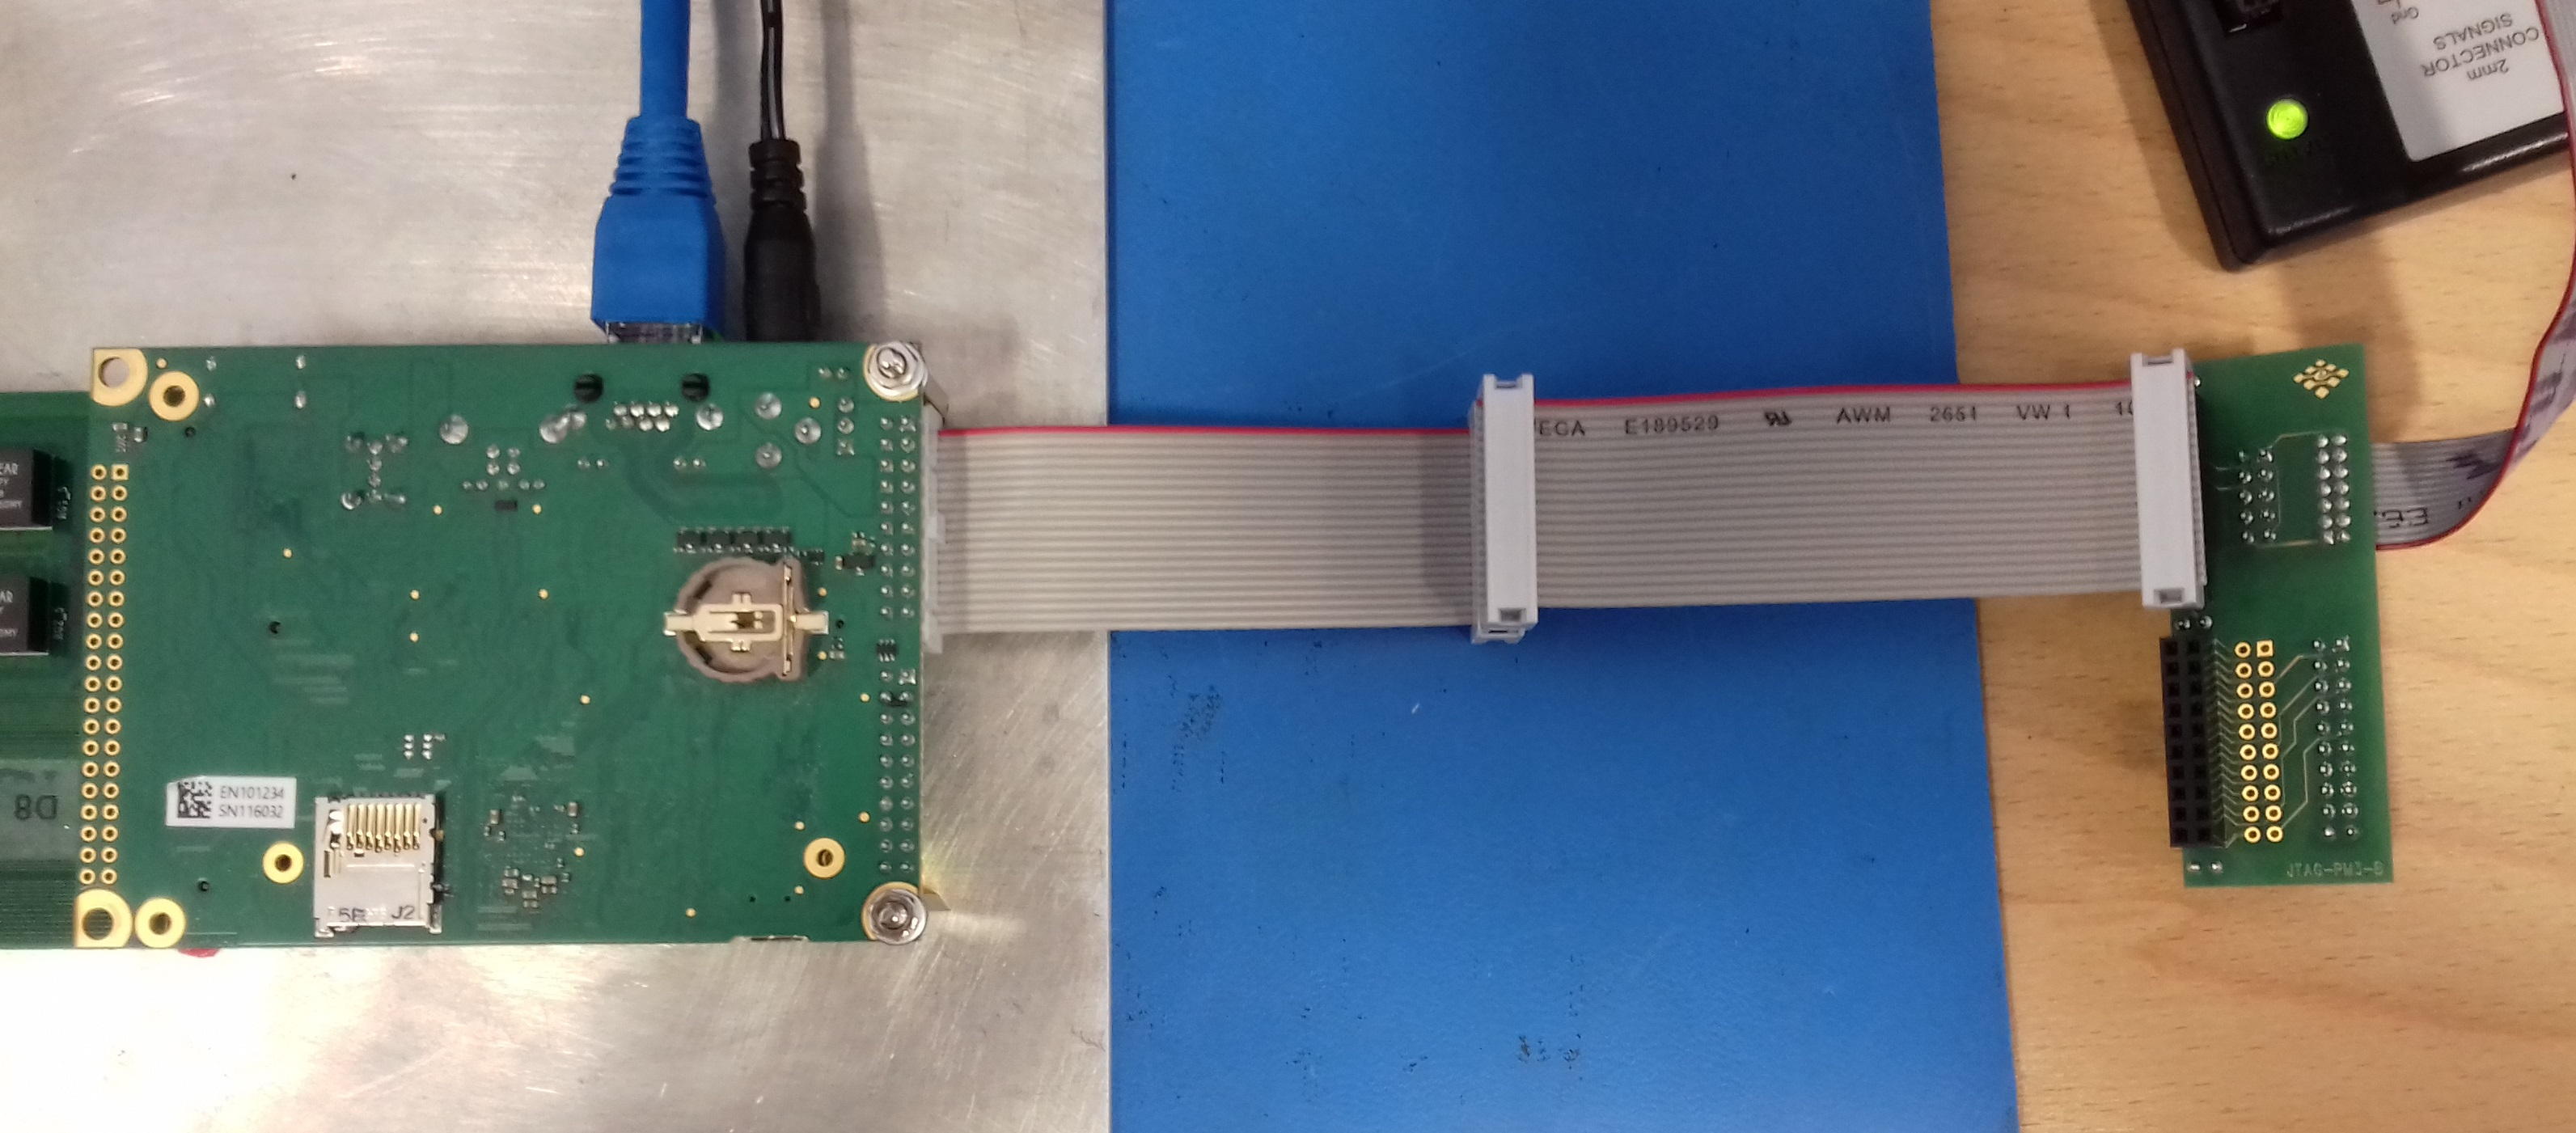
\includegraphics[width=.80\textwidth]{./Images/XilinxCable.jpg}
%  \caption{Connecting the Xilinx programming cable to the PM3 in an ugly (but effective) way.}\label{fig:XilinxCable}
%\end{figure}
